%% LyX 2.3.6.1 created this file.  For more info, see http://www.lyx.org/.
%% Do not edit unless you really know what you are doing.
\documentclass[twocolumn,english]{article}
\usepackage[T1]{fontenc}
\usepackage[latin9]{inputenc}
\usepackage{units}
\usepackage{amssymb}
\usepackage{graphicx}% Include figure files
\usepackage{dcolumn}% Align table columns on decimal point
\usepackage{bm}% bold math
\usepackage{amsmath}
\usepackage{natbib}
\usepackage{chngcntr}
\usepackage{url}
\usepackage{float}
\usepackage{fourier} 
\usepackage{array}
\usepackage{makecell}
\usepackage{background}
\usepackage[english]{babel}
\usepackage{fancyhdr}

\makeatletter

%%%%%%%%%%%%%%%%%%%%%%%%%%%%%% LyX specific LaTeX commands.
%% Because html converters don't know tabularnewline
\providecommand{\tabularnewline}{\\}

\makeatother

\pagestyle{fancy}
% \fancyhf{}
\rhead{Lab-C (TAU)}
\lhead{Spin Dependent Transport}
\renewcommand\theadalign{bc}
\renewcommand\theadfont{\bfseries}
\renewcommand\theadgape{\Gape[4pt]}
\renewcommand\cellgape{\Gape[4pt]}
\backgroundsetup{
   scale=1,
   angle=0,
   opacity=1,
   color=black,
   contents={\begin{tikzpicture}[remember picture, overlay]
      \node at ([yshift = -2.6cm] current page.north)
            {
\includegraphics[width = 3cm]{Images/logo.png}}; %
     \end{tikzpicture}}
}

\usepackage{babel}
\begin{document}
\title{Spin Dependent Transport}
\author{Alon Shaaltiel, Oren Kereth and Simon Salleh Atri}
\twocolumn[
    \begin{@twocolumnfalse}
    \maketitle
    \begin{abstract}
    By subjecting nickel, a ferromagnetic metal, to an external magnetic
    field in different orientations three effects were observed: the anomalous
    Hall effect, anisotropic magnetoresistance and the planar Hall effect.
    Using the measurements, characteristics of the crystalline structure
    of nickel were studied and also its magnetic properties were compared
    to values from the literature. 
    \end{abstract}
    \end{@twocolumnfalse}
]

\part{Theory}

\section{Magnetization}

When an external magnetic field $H$, is applied to a material, the
response of the material is called magnetic induction, $B$. The equation
relating the two is 
\begin{equation}
B=H+4\pi M\label{eq:relbetweenB=000026H}
\end{equation}
where $M$ is the magnetization of the medium and is a property of
the material. $M$  depends on moments of the atoms, ions and molecules
and their interactions as will be later explained. The ratio of $M$
to $H$ is also a property of the material as it indicates the way
the material responds to an external magnetic field  
\begin{equation}
\chi=\frac{M}{H}\label{eq: susceptibility}
\end{equation}
where $\chi$ is called the susceptibility of the material. A similar
ratio of $B$ to $H$ can also be calculated 
\begin{equation}
\mu=\frac{B}{H}\label{permeability}
\end{equation}
where $\mu$ is called the permeability of the material and indicates
how permeable the material is to a magnetic field. Some materials
have negative susceptibilities, for example, diamagnets,   upon
exertion of an external field, they reject the field by creating
a magnetization  in the opposite direction. Some materials have a
constant susceptibility (i.e. a linear relation between $H,M$) such
as paramagnets. Others have non-zero magentization with no external
field  and their susceptibility changes for different values of $H$
. Ferromagnets follow that criteria and by plotting their corresponding
$M-H$ and $B-H$ curves a  \textit{hysteresis loop} can be seen
(see Figure \ref{fig: hysteresis loop}).
\begin{figure}[H]
\includegraphics{\string"Images/Hysteresis Loop\string".jpg}\caption{Hysteresis loop of a ferromagnet \cite{SPALDIN}  \label{fig: hysteresis loop}}
\end{figure}
 Note that the changes in $M$ and in $B$ are non-linear in $H$.
Moreover, the $M-H$ curve is in this case a loop, , meaning that
for the same value of $H$ two values of $M$ are to be expected,
depending on the way the loop is traced. The magnetization also reaches
'saturation' for a sufficiently large external field as can be seen
in the edges of the loop. This saturation indicates that all the
dipoles in the material have turned  and are parallel to the external
magnetic field, yielding maximal magnetization. After reaching saturation,
the hysteresis loop shows that a non-zero external field is required
to reach $B=0$, that non-zero field, $H_{c}$, is called the coercivity
of the material. Magnets  that require a large field to do so are
called 'hard' while magnets that are easily saturated and demagnetized
are called 'soft'.

\section{Origin of Magnetization}

\subsection{Magnetic Moment of Electrons}

After analysing the macroscopic properties of ferromagnets and other
materials, let us review the microscopic origins of the magnetization.
Materials consist of atoms that are made of electrons, protons and
neutrons. The electrons are bound to the nucleus via the Coulumb interaction.
Solving the Schr{\"o}dinger equation for the bound states in a hydrogen
atom, which consists of one electron and one proton, yields the exact
 solutions
\begin{equation}
|\psi>=|nlm_{l}>\label{eq:boundstatesforhydrogen}
\end{equation}
where $n$ ,$l$ and $m_{l}$ are three quantum numbers that restrict
the energy of the bound electron, its orbital angular momentum and
the orientation of its orbital angular momentum with respect to some
magnetic field respectively. Orbitals of the electrons are named
s,p,d,f and so on, corresponding to an orbital angular momentum of
$l=0,1,2,3$ respectively. Because electrons are charged particles
that carry angular momentum they also have a magnetic moment, therefore
they generate magnetic fields and interact with magnetic fields. The
magnetic moment of the electron consists of two terms, one from its
orbital angular momentum and one from its 'internal' angular momentum-
its spin. There are two qunatum numbers relating to spin. The first
is spin quantum number, $s$,  which always equals $\frac{1}{2}$
and is analogous to the quantum number $l$. The second is $m_{s}$
which is the spin analog to $m_{l}$ and in this case is only allowed
to take the values of $\frac{1}{2},-\frac{1}{2}$. Thus, the magnetic
moment of an electron is 
\begin{equation}
\boldsymbol{m}=-g_{e}\mu_{B}m_{s}-\text{\ensuremath{\mu_{B}m_{l}}}\label{eq: electronmagneticmoment}
\end{equation}

where $\mu_{B}$ is the Bohr magneton and is defined as $\mu_{B}=\frac{e\hbar}{2m_{e}}$
where $e$,$m_{e}$ are the electron's charge and mass respectively
and $\hbar$ is the reduced Planck constant. $g_{e}$ is called the
g-factor of an electron and is approximately $2$. The total magnetic
moment of the material, made up of small electronic moments, forms
the magnetization of the material when it interacts with a magnetic
field.

\subsection{Pauli's Exclusion Principle \& Larger Atoms}

Moving to atoms containing more electrons and more protons, it is
essential to understand their energy states and how they differ from
the case of an hydrogen atom. Using perturbation theory \cite{SAKURAI}
one can find that electrons with lower angular momentum (i.e. lower
values of $l$) are lower in energy. In order to fill the unoccupied
energy states  with electrons, Pauli's exclusion principle must come
into account. Pauli's exclusion principle states that the total-electron
wavefunction (the wavefunction describing all the electrons in the
atom in this case) must be anti-symmetric with respect to any interchange
of two electrons. It can be directly inferred that no two electrons
can occupy the same state (i.e. having the exact same quantum numbers).
As a result, only two electrons may occupy each atomic orbital, one
with spin 'up' ($m_{s}=\frac{1}{2})$ and the other with spin 'down'
($m_{s}=-\frac{1}{2})$. In order to compute the total magnetic moment
of the electrons in the atom, another effect  must be taken into
account- spin orbit coupling. In short, because the electron has an
orbital momentum and there is an effective current, a magnetic field
is formed. The spin of the electron then interacts with that magnetic
field, altering the energy states and creating more favourable spin
and angular momentum states for the electrons to occupy compared to
others. 

\section{Ferromagnets}

In this section different effects contributing to ferromagnets are
explained.

\subsection{Exchange Energy}

When there is more than one electron surrounding the nucleus the Coulumb
interactions between them should be accounted for. There are two different
wavefunction configurations that are possible- one which is spatially
symmetrical under the exchange of two electrons but its spinor  is
anti symmetrical and vise-versa. Using perturbation theory to take
into account the effect of the interactions between electrons, in
the case of two electrons the energy states are
\begin{equation}
E=E_{1}+E_{2}+K\pm J\label{eq: Exchange Energy}
\end{equation}
where $E_{1},E_{2}$ are the energies of the two electrons without
the perturbation, $K$ is a perturbation term  which is not dependent
on the wave-function's configuration (i.e. the spinor's symmetry),
and the last term, $J$, is called the exchange energy,  its contribution
to the energy is dependent on the configuration of the wave-function
. $+$ is for the configuration of two anti-parallel spins (anti-symmetrical
spinor) and $-$ is for the configuration of two parallel spins (symmetrical
spinor). The implication of this result is that one spin configuration
is more favourable compared to the other. In the case of $J>0$ the
electrons will prefer to align their spins as it is more energetically
favourable, yielding spontaneous magnetization without any external
field. However, there are more effects taking place that need to be
taken into account.

\subsection{Collective Electron Theory of Ferromagnetism}

The alignment of electrons in the same direction is opposed by the
band energy involved in transferring electrons from the lower energy
states that are  entirely occupied to the higher energy states that
are partially occupied. In ferromagnets, the Fermi energy  lies in
a region of overlapping 3d and 4s states. Due to the high density
of states near the Fermi level in the 3d orbital and the low density
in the 4s orbital, the 3d states are effected by exchange interactions
while 4s states are not.  Therefore there is a preferred spin alignment
. Because there is exchange splitting in that region and the 3d orbital
is only partially occupied, there will be spontaneous magnetic moment
(and therefore it is a ferromagnet). If the Fermi energy lies above
the 3d orbital, despite the exchange interaction taking place in the
3d orbital, all 3d states will be filled with down and up spin electrons,
thus negating the magnetic moment. The difference in the Fermi energy
can make the difference between a ferromagnet and a simple metal.


\subsection{Domains}

Despite the exchange interaction that suggests that ferromagnets should
be magnetized with all of the electrons having the same parallel spin,
they are not. Instead, ferromagnetic domains are formed, where all
the spins are aligned parallel to each other . The average magnetization
is therefore 0. The domains are formed in order to minimize other
contributions to the total magnetic energy.

\subsubsection{Magnetostatic Energy}

If all the spins in the material were parallel to each other, a large
magnetic field would have formed, with a corresponding energy of
\begin{equation}
U_{H}=\frac{1}{4\pi}H_{d}^{2}\label{eq: Magnetostatic Energy}
\end{equation}
where $H_{d}$ is called the demagnitizing field and is essentially
the field created by the magnetized ferromagnet. $U_{H}$ is the energy
stored in that demagnetizing field (maybe refernce griffith or something
idk). By forming more domains with different spin alignments, the
demagnetizing field is reduced, thus minimizing the magnetostatic
energy while maximizing the exchange energy in each domain  (see
Figure \ref{fig: magnetostatic energy}).
\begin{figure}[H]
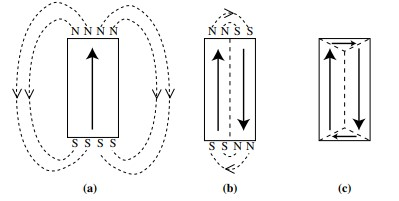
\includegraphics[scale=0.75]{Images/Magnetostatic}

\caption{Reduction of the magnetostatic energy by domain formation \cite{SPALDIN}
\label{fig: magnetostatic energy}}
\end{figure}
 The shape of the domains and their orientation is also dependant
on the magnetocrystalline energy and magnetostrictive energy.

\subsubsection{Magnetocrystalline Energy}

The magnetization in ferromagnetic crystals tends to align along certain
preferred crystallographic directions. The preferred directions are
called the \textquotedblleft easy\textquotedblright{} axes, since
it is easiest to magnetize a demagnetized sample to saturation if
the external field is applied along a preferred direction \cite{SPALDIN}
and the ``hard'' axes are those that require the most energy in
order to magnetize (i.e. larger external field to reach saturation).
The energy difference per unit volume between samples magnetized along
easy and hard axis is called the magnetocrystalline anisotropy energy.
In order to minimize the magnetocrystalline energy, the domains will
form such that their spins point along easy axis. Within the interface
between domains  the direction of magnetization changes, and therefore
cannot be aligned along an easy axis, thus increasing the energy.
Therefore, the magnetocrystalline energy favors a few domains with
less boundaries over many domains with many boundaries .

\subsubsection{Magnetostrictive Energy}

When a ferromagnetic material is magnetized it undergoes a change
in length known as magnetostriction. Domains with different orientations
that are near each other cannot elongate at the same time, for example,
in figure 2 the vertical and horizontal domains are unable to elongate
simultaneously along their corresponding spin directions. As a result,
an elastic strain energy term is added to the total energy. This energy
favors small closure domains and therefore favors many small domains.
The domains are thus formed as an optimization of the energies above.

\section{Ferromagnetic Effects}

Due to the nature of ferromagnets, some unusual  effects regarding
the resistance of the ferromagnet can be measured. This experiment
will revolve around these important effects.

\subsection{Hall Effect}

Suppose there is a block of metal (see Figure \ref{fig: Ohm's Law})
, by applying an electric field in the $x$ direction (using a battery
with some known voltage $V_{x}$) an electric current $I$ with a
corresponding current density $J_{x}$ starts flowing through the
metal in the same direction.
\begin{figure}[H]
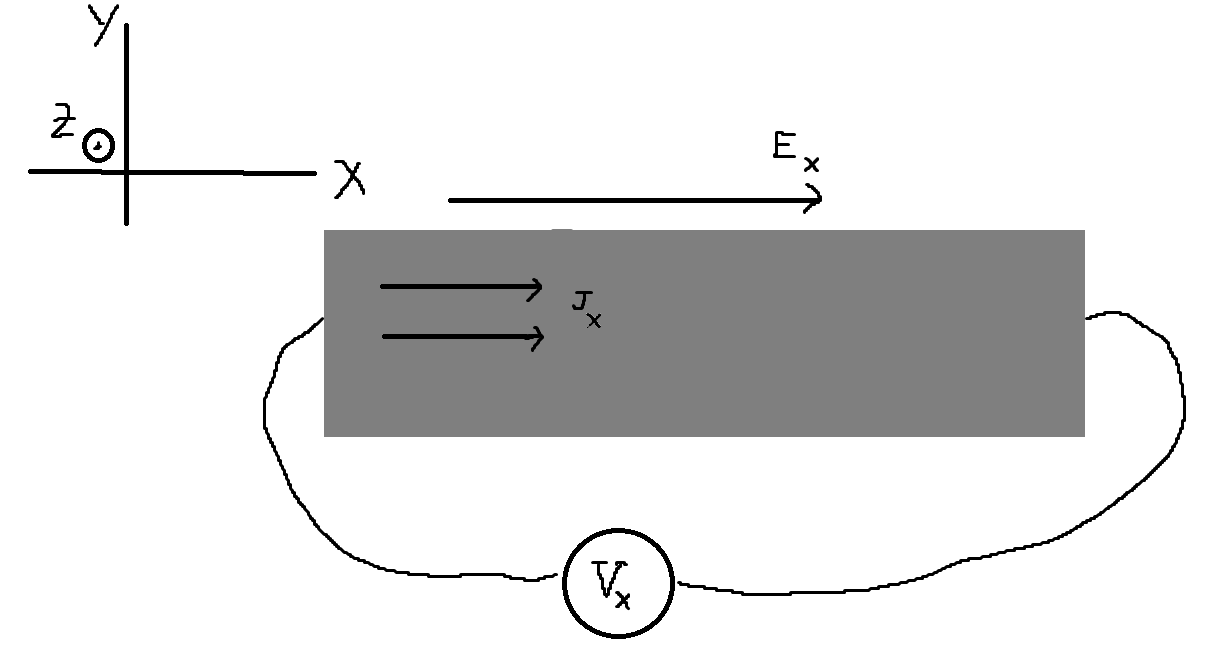
\includegraphics[scale=0.25]{Images/HallEffectnomagnet}

\caption{Ohm's Law. An electric field $E_{x}$ generates current density $J_{x}$
in a block of metal \label{fig: Ohm's Law}}
\end{figure}
This is Ohm's law which can also be derived from Drude's equation
\cite{StevenSimon}. Now, suppose a magnetic field, $H$, is applied
in the z direction in addition to the existing electric field. The
magnetic field will interact with the flowing electrons through Lorentz
force and deflect the electrons to the $y$ direction. As a result,
negatively charged electrons  will accumulate on one side of the
metal block while the other side will become positively charged due
to the vacant electrons. These charges  will then generate an electric
field in the $y$ direction, $E_{y}$, and in a steady state a voltage
can be measured in that direction (see Figure \ref{fig: Hall Effect}).
\begin{figure}[H]
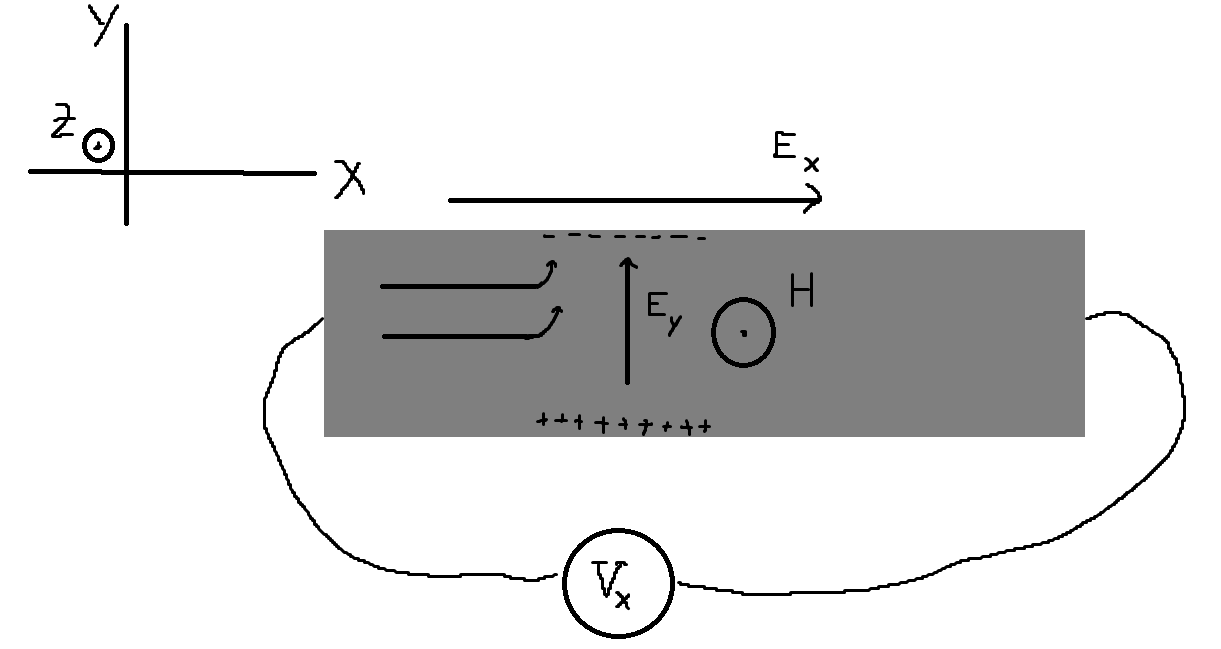
\includegraphics[scale=0.25]{Images/HallEffectwithmagnet}

\caption{Hall Effect. The magnetic field creates a measurable voltage in the
$y$ direction. \label{fig: Hall Effect}}
\end{figure}
The electric field in the $y$ direction and the current density $J_{x}$
are related through the Hall coefficient 
\begin{equation}
E_{y}=R_{H}HJ_{x}\label{eq: Hall Effect}
\end{equation}
where $R_{H}$ is the Hall coefficient and is defined as 
\begin{equation}
R_{H}=-\frac{1}{ne}\label{eq: Hall Coefficient}
\end{equation}
where $e$ is the charge of the electron and $n$ is the charge density.
It is important to note that this effect is negative for positive
magnetic fields, meaning that if $R_{xy}\equiv\frac{V_{y}}{I_{x}}$
is measured and is plotted against the magnetic field $H$, a linear
curve with a negative slope is to be expected. This linear curve is
anti-symmetrical for the exchange of $H\rightarrow-H$.

\subsection{Anomalous Hall Effect}

While The Hall effect can be measured in simple metals, the anomalous
Hall effect (AHE) is unique to ferromagents. Suppose the metal block
from the previous section is now a ferromagnetic plate and magnetized
in a direction perpendicular to the plane of the plate. A current
is passed through the plate in the $x$ direction and the electrons
in the current  be scattered by the magnetized atoms. The scattering
will turn out to be asymmetrical as explained later in this section.
As a result a charge will build up on the edges of the plate, creating
an electric field in the $y$ axis according to 
\begin{equation}
E_{s}=R_{s}MJ_{x}\label{eq: Anomolous Hall Effect}
\end{equation}
where $E_{s}$ is the electric field in the $y$ axis, $M$ is the
magnetization of the plate and $R_{s}$ is referred to as the anomalous
Hall coefficient. The anomalous Hall resistivity is far greater by
magnitude than the normal Hall effect. \newpage Let us explain the
anomalous Hall effect using a microscopic analysis of the conductance
band and its overlapping part with the 3d shell. As mentioned in a
previous section, the 3d orbital is effected by the exchange interaction
due to the dense energy states, thus a clear split between up and
down spin electrons in this orbital occurs, with parallel spin electrons
being a more energetically favourable configuration until the energy
gaps force otherwise. The spin up electrons are shifted down while
the spin down electrons are shifted up. In addition to the exchange
interaction affecting the d-states, spin-orbit coupling creates further
divisions as it removes the degeneracy of different $m_{l}$ values
for the spin up and down electrons (see Figure \ref{fig: AHEEXPLAINED}
)
\begin{figure}[H]
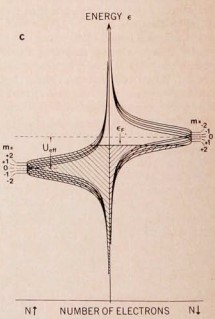
\includegraphics{Images/AHEExplained}

\caption{Density of states for the d-level of a ferromagnet \cite{BERGMAN}
 \label{fig: AHEEXPLAINED}}
\end{figure}
In the case shown in the figure, with the Fermi energy being where
it is, the spin up states are nearly filled whereas the spin down
states are filled only for the $m=2$ states, therefore the conduction
electrons flowing through the metal have a far greater chance to be
scattered into one of the $m=2$ states than into the $m=-2$, creating
an asymmetric scattering which gives rise to the anomalous Hall effect.
If the Fermi level lies above the maximum of the spin-down resonance
the density of $m=-2$ states exceeds that of $m=+2$ states, and
the asymmetry in the scattering changes its sign. This is the case
in Nickel, the metal we are working with in this experiment, and
so the anomalous Hall resistance is negative for positive magnetization
(parallel to the $z$ axis) . In Nickel, combining the anomalous
Hall effect with the normal Hall effect explained in the previous
section, the total resistivity $R_{xy}$ as defined previously, increases
in magnitude for increasing external magnetic fields due to the two
Hall coefficients sharing the same negative sign (whereas for iron,
whose Fermi energy lies below the maximum of spin down resonance the
two effects interfere with one another). This phenomenon will be shown
later in this report. Due to the dependency of the AHE in the magnetization
of the ferromagent, it reaches saturation once the magnetization reaches
saturation, and an hysteresis loop is formed for the resistivity just
as it is formed for the magnetization $M$. Therefore, by looking
at the Hall resistivity curve information about the material and its
magnetization properties can be extracted as will be seen in later
sections of this report.

\subsection{Anisotropic Magnetoresistance (AMR)}

AMR is the change in resistance when a magnetic field is applied on
a ferromagnetic metal or alloy, the change depends on the direction
of the field relative to the current and is therefore anisotropic.
Non-ferromagnetic metals also change their resistance under a magnetic
field, this effect is called magnetoresistance (MR) and is much weaker.
As the MR in a ferromagnetic metal is almost entirely from AMR, other
sources of MR are not accounted for.

The origin of AMR is the spin--orbit coupling, the s electrons which
are responsible for the conduction are scattered by the vacant part
of the orbital angular momentum of the 3d electrons. As the magnetization
direction rotates in response to the applied magnetic field, the 3d
electron cloud deforms, and changes the amount of scattering of the
conduction electrons. When the magnetization direction is perpendicular
to the current direction, the scattering cross-section is reduced
compared with the zero-field case, whereas when the magnetization
direction is parallel to the current direction, the scattering cross-section
is increased. This concept is illustrated in Figure \ref{fig: AMR_Schematic}.

\begin{figure}[H]
\includegraphics[scale=0.35]{\string"Images/AMR Schematic\string".png}

\caption{An illustrated representation of the AMR process \cite{SPALDIN}.
\label{fig: AMR_Schematic}}
\end{figure}

The resulting effect on the measured magneto resistance is illustrated
in Figure \ref{fig: AMR_MagnetoResistance}.

\begin{figure}[H]
\includegraphics[scale=0.5]{\string"Images/AMR Graph\string".png}

\caption{The changes to the magnetoresistance depending on the field's direction
in reference to the current \cite{SPALDIN}. \label{fig: AMR_MagnetoResistance}}
\end{figure}


\subsection{Planar Hall Effect (PHE)}

Suppose there is a plate made out of a ferromagnetic material, an
external magnetic field is exerted in the same plane as the plate
and current is flowing through the plate in some direction $\hat{n}$
. The angle between the magnetic field and $\hat{n}$ is $\theta$,
if $\theta=0$ the effect detailed in the AMR section for  a parallel
field will occur  and the resistance  will be higher than without
the  field. If $\theta=\frac{\pi}{2}$ then the magnetic field will
be perpendicular, lowering the resistance. For a general angle the
resistance parallel to the current , denoted $R_{xx}$ can be expressed
as 
\begin{equation}
R_{xx}=\rho_{par}cos^{2}\theta+\rho_{perp}sin^{2}\theta\label{eq: PHE - RXX}
\end{equation}
where $\rho_{par}$ is the resistance in the case of a parallel magnetic
field (when $\theta=0$ $R_{xx}=\rho_{par}$) and $\rho_{perp}$ is
the resistance in the case of a perpendicualr magnetic field (when
$\theta=\frac{\pi}{2}$). For the resistance in the direction perpendicular
to current flow, denoted by $R_{xy}$, there is a similar relation
\begin{equation}
R_{xy}=\frac{\rho_{perp}-\rho_{par}}{2}sin(2\theta)\label{eq: PHE- RXY}
\end{equation}
These two expression can be found using the resistibility matrix and
applying rotations on it. This matrix in the case of a parallel field
($\theta=0)$ is
\begin{equation}
\rho_{0}=\begin{bmatrix}\rho_{par} & 0\\
0 & \rho_{perp}
\end{bmatrix}\label{eq: PHE- resistibility matrix}
\end{equation}
Where the diagonal elements are $R_{xx}$ and $R_{yy}$ for the two
distinct cases of current flowing in $\hat{n}$ or perpendicular to
it respectively. If the current is perpendicular to $\hat{n}$ it
is also perpendicular to the magnetic field and thus $R_{xy}=\rho_{perp}$
in this case . In order to find the resistibility matrix for a general
angle $\theta$, this matrix should be rotated using a rotation matrix
around the $z$ direction. After rotating,  the resistibility matrix
turns out to be

\begin{multline}
\rho_{planar}(\theta)=R^{-1}\rho_{0}R=\\
\begin{bmatrix}\rho_{par}cos^{2}\theta+\rho_{perp}sin^{2}\theta & \frac{\rho_{par}-\rho_{per}}{2}sin(2\theta)\\
\frac{\rho_{par}-\rho_{per}}{2}sin(2\theta) & \rho_{perp}cos^{2}\theta+\rho_{par}sin^{2}\theta
\end{bmatrix}\label{eq: PHE - RESISTIBILITY MATRIX AFTER ROTATION}
\end{multline}

In this part of the experiment the resistibility matrix will be found
by exerting a constant magnetic field and changing its angle compared
to the sample.

\part{Experimental Setup}

As previously mentioned, in this experiment we will be using a nickel
plate whose curie temperature is well above room temperature \cite{NICKELCURIETEMP},
and therefore will be in its ferromagentic phase in all the following
measurements. This nickel plate has a known thickness of $10nm$ and
is deposited on a crystal substrate which is mounted on a chip carrier
(see Figure \ref{fig:SchematicofChip}).
\begin{figure}[H]
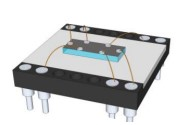
\includegraphics{Images/NickelandtheChip}

\label{fig:SchematicofChip}\caption{The experimental setup- schematic of the sample and the chip carrier}
\end{figure}
The chip carrier is connecting into a rotating base and inserted into
an electromagnet. The chip carrier is connected to a multimeter that
can perform a 4 probe measurement (see Figure \ref{fig:electromagnetandrotatingbase})
\begin{figure}[H]
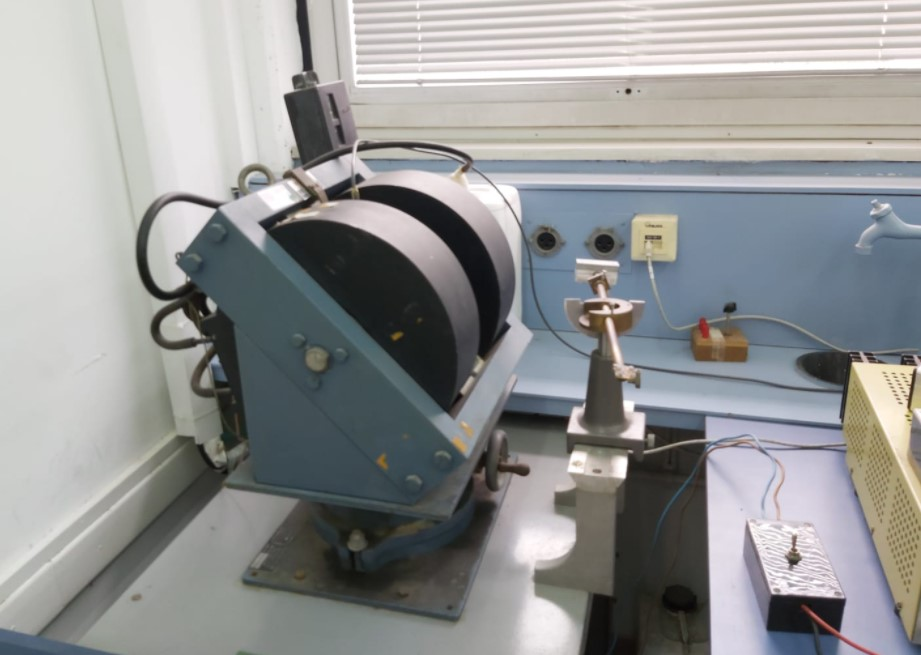
\includegraphics[scale=0.25]{Images/ExperimentalSystem-ElectroMagnet}

\caption{The experimental setup- electronmagnet and rotating base \label{fig:electromagnetandrotatingbase}}
\end{figure}
 Using a Lakeshore Model 425 Gaussmeter, the magnetic field applied
by the electromagnet was be measured. The magnetic field is created
using current flowing through coils, the current can be changed and
its direction can be reversed using a button. Throughout this experiment,
the resistance of the nickel sample in any given direction was be
measured simultaneously with the magnetic field.

\section{AHE}

In this part of the experiment we are interested in $R_{xy}$. The
magnetic field was changed and the resistance perpendicular to the
direction of flow was measured. Using these measurements information
regarding nickel's ferromagnetic properties was extracted, as will
be further explained later in this report. By measuring both the anomalous
and normal Hall effects and using the known values of $R_{s}$ for
nickel its saturation magnetization and charge carrier density were
extracted as well. In order to create AHE the magnetic field was applied
perpendicular to the current flow direction with magnitudes ranging
between $-4300\,[Gauss]$ and $4300\,[Gauss]$ .

\section{PHE}

In this part of the experiment, the magnetic field was applied in
the same plane as the current's flow direction and $\theta$ , the
angle between the current flow direction and the applied field was
changed by rotating the base. For each angle the resistance both in
the current flow direction and perpendicular to it was measured and
the magnitude of the magnetic field remained constant throughout this
experimental section. Using these measurements the resistivity matrix
from equation \ref{eq: PHE - RESISTIBILITY MATRIX AFTER ROTATION}
of the sample was extracted.

\section{AMR }

In this part of the experiment the resistance was measured parallel
to the current's flow direction. The magnetic field was be applied
in different directions and the change in resistance correlating to
each direction and magnitude and magnetic field was measured. The
expected results can be seen in Figure \ref{fig: AMR_MagnetoResistance}.
The magnetic field was applied perpendicular to the current, transverse
to it and parallel to it. The change in saturation resistance (where
the magnetization reaches saturation) between magnetic field direction
was extracted using the measurements 
\begin{equation}
\frac{\Delta\rho}{\rho}\equiv\frac{\rho_{per}-\rho_{par}}{\rho_{avg}}\label{eq: AMR comparison between directions}
\end{equation}
where $\rho_{per}$ is the saturation resistance when the magnetic
field was perpendicular to the current, $\rho_{par}$ when the magnetic
field was parallel and $\rho_{avg}$ is the average of all resistances
with all magnetic field directions for the saturated nickel. Similarly
to the previous part, information regarding the ferromagentic properties
of nickel such as its easy axis and more  was extracted using these
measurements.

\part{Measurements}

\global\long\def\ten#1{\times10{}^{#1}}%


\section{AHE}

By changing the magnetic field perpendicular to the sample and measuring
the resistance perpendicular to the current flow, a hysteresis loop
was traced due to the relation of AHE with the magnetization of the
material. The saturation resistance (for which AHE saturates and the
normal Hall effect starts to dominate) was found by fitting pairs
of linear fits, one fit was made after saturation, where the change
in resistance is linear due to the normal Hall effect. The other linear
fit was made before saturation but using measurements close enough
to the approximated region. The saturation resistance was then approximated
as the average intersection point of the linear fits (see Figure \ref{fig: AHE linear fits})
\begin{figure}[H]

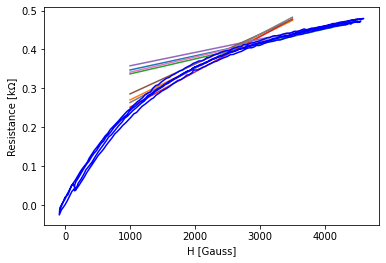
\includegraphics[scale=0.6]{Images/AHElinearfits}\caption{Linear fits at the saturation region \label{fig: AHE linear fits}
}
\end{figure}
 Using that saturation resistance and the known thickness of the sample,
the saturation magnetization of the sample was found using the equation
\begin{equation}
\rho_{H}=\frac{R_{0}H+4\pi R_{s}M_{s}}{t}\label{eq: AHE saturation magnetization equation with the thickness}
\end{equation}
where $t=10nm$ is the thickness of the nickel sample, $M_{s}$ is
the magnetization of the nickel which we are interested in, $\rho_{H}$
is the resistivity of the sample extracted from the measurements and
$R_{0}$ is a constant resistance. The saturation magnetization came
out to be 
\begin{equation}
M_{saturation}=4.01\times10^{3}\pm2.3\times10^{2}(5.7\%R.E)\unitfrac{emu}{cm^{3}}\label{eq: SaturationMagnetizationofNickelAHE}
\end{equation}
Furthermore, using the linear region where the normal Hall effect
dominates, the normal Hall coefficient was extracted, from which the
charge carrier density was extracted using the relation 
\begin{equation}
R_{0}=\frac{1}{ne}\label{eq: relation between hall coefficient and charge carrier density}
\end{equation}
where $n$ is the charge carrier density and $e$ is the charge of
the electron. The charge carrier density came out to be
\begin{equation}
n=1.5601752\times10^{24}\pm9.3\times10^{18}(0.00060\%)\frac{1}{m^{3}}\label{eq: charge carrier density}
\end{equation}
The saturation susceptibility of nickel calculated in CGS turned out
to be
\begin{equation}
\chi_{sat}=\frac{M_{sat}}{H_{sat}}=18.0\pm1.4(7.6\%)\label{eq: susceptibilityofNICKEL}
\end{equation}
This value is of the same scale as that taken from the literature
\cite{NICKELSUSCEP}. Using the measurements, the coercivity of nickel
in the measured axis was found to be 
\[
H_{C}=30G
\]
which is in agreement with theoretical values \cite{stupidarticle}.
The susceptibility could not be measured prior to saturation due to
the hysteresis loop that yields two different magnetization values
for every external field, therefore $\chi$ is undefined.

\section{PHE }

Measurements of $R_{xy}$ and $R_{xx}$ were made for 38 different
angles in the range $[0,\pi]$ with a constant external magnetic field
$H=3493G$ . $R_{xx}$ and $R_{xy}$ were fitted according to equations
\ref{eq: PHE - RXX} and \ref{eq: PHE- RXY} in the following manner:
$R_{xx}$ was fitted to the function
\[
y=a_{0}cos^{2}(2x)+a_{1}sin^{2}(2x)
\]
where $a_{0}$ has the theoretical value $\rho_{par}$ and $a_{1}$
has the theoretical value $\rho_{perp}$. $R_{xy}$ was then fitted
to the function 
\[
y=b_{0}sin(2x)+b_{1}
\]
where $b_{0}$ is expected to be $\frac{\rho_{par}-\rho_{perp}}{2}$
extracted from the previous fit . The fit for $R_{xx}$ yielded the
following results (see Figure \ref{fig: RXX FIT}):
\begin{figure}[H]
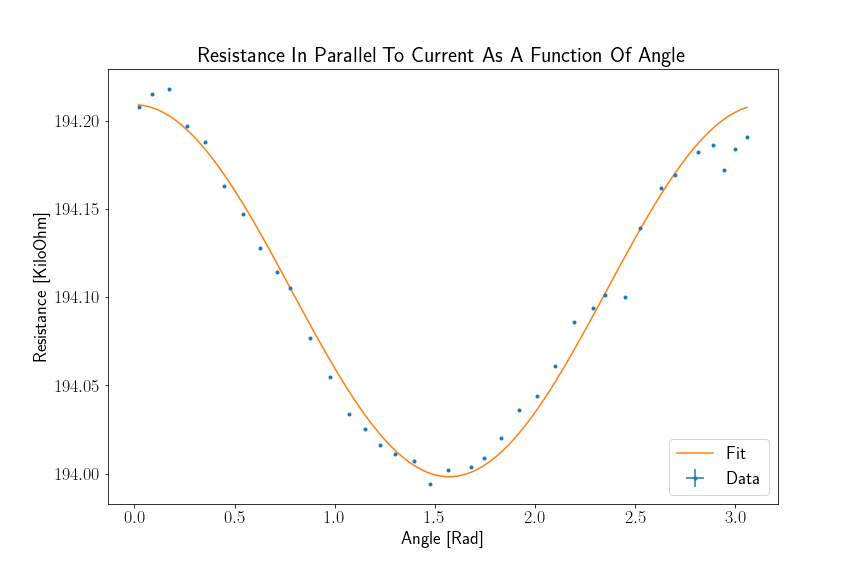
\includegraphics[scale=0.25]{Measurements/PHE/Rxx_Plot}\caption{$R_{xx}$ as a function of the angle between the magnetic field and
current flow direction, $\theta$ \label{fig: RXX FIT}}
\end{figure}
 The corresponding fit parameters and statistical values are presented
in Table \ref{tbl: Rxx fit parameters}.
\begin{table}[H]
\begin{tabular}{|c|c|c|}
\hline 
Parameter & Value & Error (Relative Error)\tabularnewline
\hline 
\hline 
$a_{0}[k\Omega]$ & $1.942\ten 2$ & $2.42\ten{-3}$($0.0012\%)$\tabularnewline
\hline 
$a_{1}[k\Omega]$ & $1.940\ten 2$ & $2.45\ten{-3}$($0.0013\%)$\tabularnewline
\hline 
$\chi_{red}^{2}$ & $2.8\ten 4$ & -----------\tabularnewline
\hline 
$p_{value}$ & $0.0$ & -----------\tabularnewline
\hline 
\end{tabular}

\caption{$R_{xx}$ fit parameters and statistical values \label{tbl: Rxx fit parameters}}
\end{table}
Using the fit parameters and according to equation \ref{eq: PHE - RXX}
$\rho_{par}$ and $\rho_{perp}$ were both extracted 

\begin{multline}
\rho_{par}=1.942\ten 2\pm2.42\ten{-3}(0.0012\%)[k\Omega]\\
\rho_{perp}=1.940\ten 2\pm2.45\ten{-3}(0.0013\%)[k\Omega]\label{eq: Rxx extracted values}
\end{multline}

The statistical values are out of their corresponding desired ranges,
however, the fit shows that the function the data was fitted to describes
the phenomena adequately with some needed tweaks as the residuals
plot shows a clear trend of some high order polynomial as can be seen
in Figure \ref{fig: Rxx residuals plot}
\begin{figure}[H]
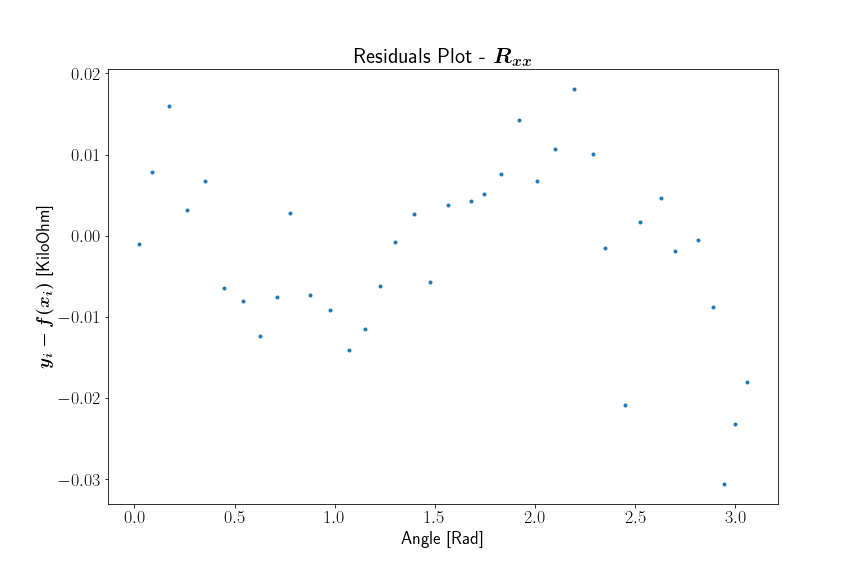
\includegraphics[scale=0.25]{Measurements/PHE/Rxx_Res}\caption{Residuals plot of the $R_{xx}$ fit \label{fig: Rxx residuals plot}}

\end{figure}
Further discussion is on later sections of this report. For $R_{xy}$
the fit yielded the following results (see Figure \ref{fig: RXY FIT}):
\begin{figure}[H]
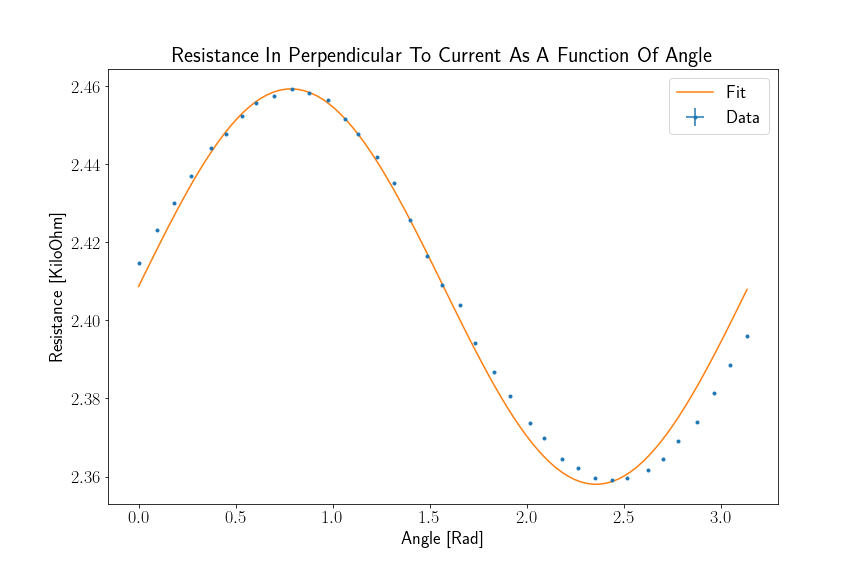
\includegraphics[scale=0.25]{Measurements/PHE/Rxy_Plot}\caption{$R_{xy}$ as a function of the angle between the magnetic field and
current flow direction, $\theta$ \label{fig: RXY FIT}}
\end{figure}
 The corresponding fit parameters and statistical values are presented
in Table \ref{tbl: Rxy fit parameters}
\begin{table}[H]
\begin{tabular}{|c|c|c|}
\hline 
Parameter & Value & Error (Relative Error)\tabularnewline
\hline 
\hline 
$b_{0}[k\Omega]$ & $5.067\ten{-2}$ & $7.4\ten{-4}$($1.4\%)$\tabularnewline
\hline 
$b_{1}[k\Omega]$ & $2.40868$ & $6.0\ten{-4}(0.025\%)$\tabularnewline
\hline 
$\chi_{red}^{2}$ & $7.9\ten 3$ & -----------\tabularnewline
\hline 
$p_{value}$ & $0.0$ & -----------\tabularnewline
\hline 
\end{tabular}

\caption{$R_{xy}$ fit parameters and statistical values \label{tbl: Rxy fit parameters}}
\end{table}
Similar to the previous fit, the statistical values are out of their
corresponding desired ranges, yet the fit shows that the function
the data was fitted to describes the phenomena adequately with some
needed tweaks as the residuals plot shows a clear trend of some high
order polynomial as can be seen in Figure \ref{fig: Rxy residuals plot}
\begin{figure}[H]
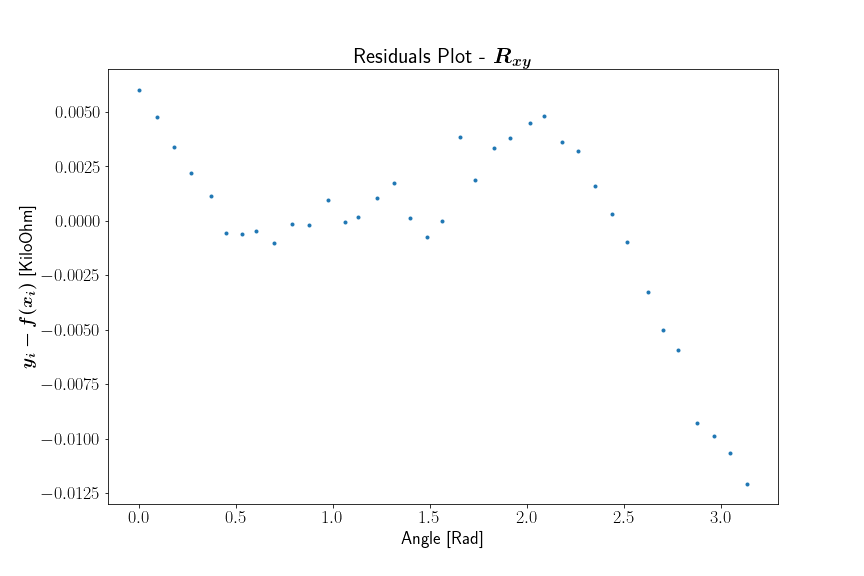
\includegraphics[scale=0.25]{Measurements/PHE/Rxy_Res}\caption{Residuals plot of the $R_{xy}$ fit \label{fig: Rxy residuals plot}}
\end{figure}
Similar problems occur for both fits. More about it in the discussion.

\section{AMR }

Measurements of the resistance in parallel to the current ($R_{xx}$)
were collected while the external magnetic field was cycling from
$-4300\,[Gauss]$ to $4300\,[Gauss]$. The external field was oriented
in parallel, perpendicular and transversely to the current. The AMR
effect is symmetric to a $180^{\circ}$ rotation of the external field
and so, the measurements were separated into the symmetric and anti-symmetric
parts, as any function can be

\textbf{\emph{
\[
f(x)=\underbrace{\frac{f(x)+f(-x)}{2}}_{\text{symmetric}}+\underbrace{\frac{f(x)-f(-x)}{2}}_{\text{anti-symmetric}}
\]
}}

The symmetric part includes the expected AMR effects on the resistance
while the anti-symmetric part includes the temperature dependence
and other effects such as AHE which occurs due to the $R_{xy}$ contribution to the resistance, as it is not entirely parallel.
To accurately find $R(H)$ and $R(-H)$
pairs ($R$ denotes resistance, $H$ denotes the applied field), evenly
distanced measurements were interpolated on both positive and negative
field values, such that both sides had the same number of measurements
and at opposite fields. As there are multiple different measurements
going from one end to the other in each run, the measurements were
broken up into ``tracks'' of single measurements from $-4300\,[Gauss]$
to $4300\,[Gauss]$, each track has its own symmetric and anti-symmetric
parts.

The average resistance of the symmetric part at saturation was calculated.
Points were selected depending on their distance (in standard deviations)
from previous nearby points and the average. These averages represent
$\rho_{Perpendicular}$ ($\rho_{P}$), $\rho_{Transverse}$ ($\rho_{T}$)
and $\rho_{Parallel}$ ($\rho_{\parallel}$), each corresponding to
its respective measurement, see Figures \ref{fig: AMR_PerpSymResistance}
through \ref{fig: AMR_ParSymResistance}.

\begin{figure}[H]
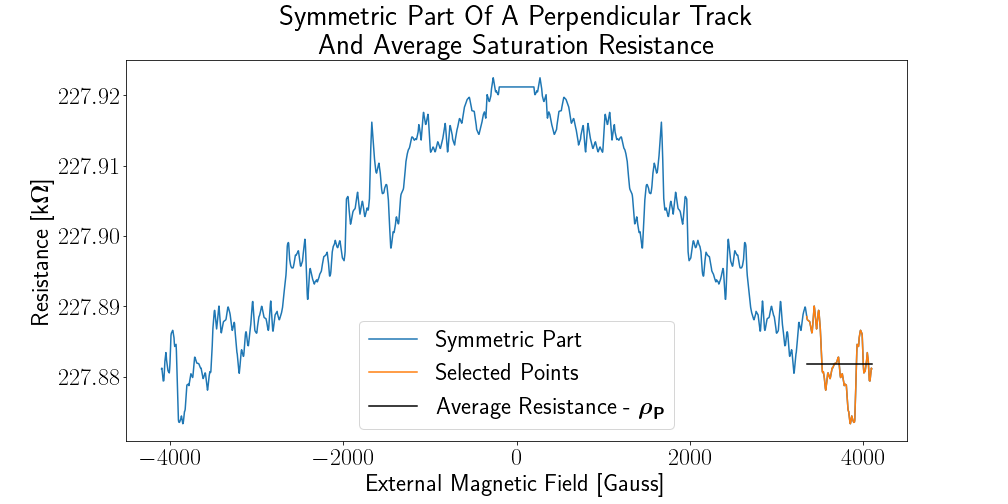
\includegraphics[scale=0.25]{Measurements/AMR/PerpendicularResistance}

\caption{The extracted symmetric part of the first track for measurements with
a perpendicular external field and the average resistance at saturation.
\label{fig: AMR_PerpSymResistance}}
\end{figure}
\begin{figure}[H]
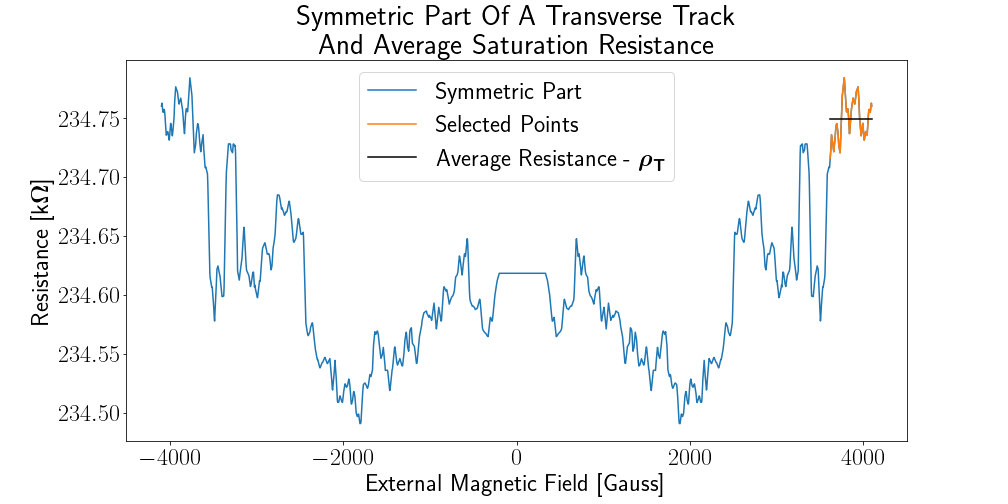
\includegraphics[scale=0.25]{Measurements/AMR/TransverseResistance}

\caption{The extracted symmetric part of the second track for measurements
with a transverse external field and the average resistance at saturation.
\label{fig: AMR_TransSymResistance}}
\end{figure}
\begin{figure}[H]
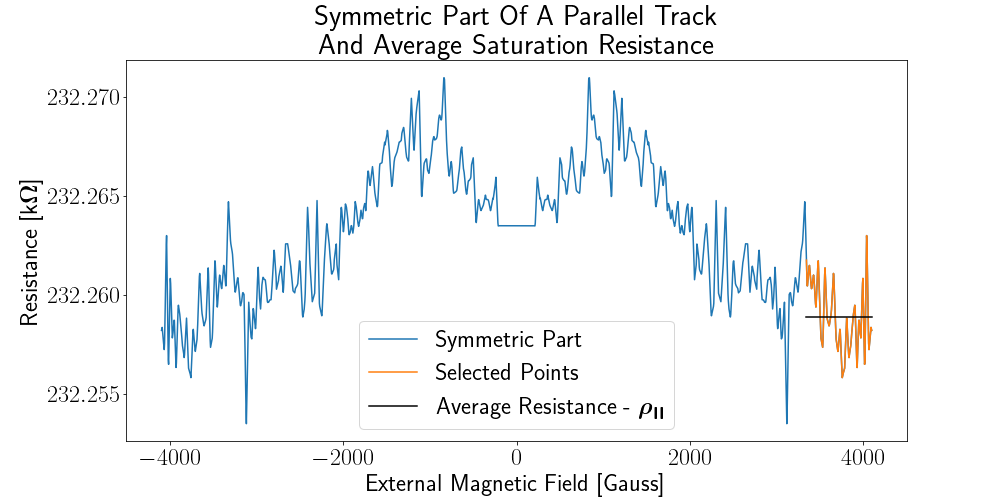
\includegraphics[scale=0.25]{Measurements/AMR/ParallelResistance}

\caption{The extracted symmetric part of the first track for measurements with
an external field parallel to the current and the average resistance
at saturation.\label{fig: AMR_ParSymResistance}}
\end{figure}

The average resistances are presented in Table \ref{tab: AMR_AverageResistances}.

\begin{table}[H]
\begin{tabular}{|c|}
\hline 
Average Resistance In Each Orientation (R.E.)\tabularnewline
\hline 
\hline 
$\rho_{P}=2.3225890\ten 2\pm1.1\ten{-4}\,(4.7\ten{-5}\%)\,[k\Omega]$\tabularnewline
\hline 
$\rho_{T}=2.2788180\ten 2\pm3.1\ten{-4}\,(1.36\ten{-4}\%)\,[k\Omega]$\tabularnewline
\hline 
$\rho_{\parallel}=2.347496\ten 2\pm1.5\ten{-3}\,(6.4\ten{-4}\%)\,[k\Omega]$\tabularnewline
\hline 
\end{tabular}

\caption{Average resistances at saturation for different field orientations
\label{tab: AMR_AverageResistances}}
\end{table}

The resistances are of the same order as those extracted in PHE. 
\global\long\def\r{\rho}%

The metric $\frac{\Delta\r}{\r}=\frac{2|\r_{P}-\r_{\parallel}|}{\r_{P}+\r_{\parallel}}=1.1\%$
shows the scale of the AMR effect to be a small percentage of the
total resistance.

More on the graphs, and resistances in the discussion.

\part{Discussion}

Please note the change in order, AHE's discussion is last.

\section{PHE}

In this section of the experiment the magnetic field was applied in
the same plane as the nickel plate and the angle between the current
flow direction and the external magnetic field was changed from the
values 0 to $\pi$. Two fits were made according to equation \ref{eq: PHE - RESISTIBILITY MATRIX AFTER ROTATION}
to $R_{xx}$ and $R_{xy}$ from which $\rho_{par}$ and $\rho_{perp}$
were both extracted. The relative errors on both values came out low,
which can perhaps be attributed to not taking larger errors on the
measurements. Regardless, the statistical values are not in their
desirable ranges and a clear trend can be seen in both residuals plots.
However, the behavior of the measurements matches that described by
the theory, sine and cosine function do seem, for the most part to
describe the phenomena. In addition to that, for $\theta=0,\pi$ a
clear maximum in the resistance be seen, matching the fact that $\rho_{par}>\rho_{perp}$
as explained in the AMR theoretical section. Similarly, for $\theta=\frac{\pi}{2}$
a clear minimum can be seen, fitting the same explanation given in
the AMR section. In search for possible sources that could have altered
the measurements and led to the inadequate fits a few ideas came up.
First of all, the external magnetic field changes with time and the
fluctuations are not random. This can also be seen in Figure \ref{fig: Magneticfieldfluctuations}
where the fluctuations seem to change periodically with time with
a small amplitude of $50G$ .
\begin{figure}[H]
\includegraphics[width=\linewidth]{\string"Measurements/Graphs/Field Flactuations\string".png}

\caption{Field fluctuations in the magnetic field \label{fig: Magneticfieldfluctuations}}

\end{figure}
This change might not be powerful on its own to alter measurements
(as they were measured in only slightly different external magnetic
fields) but can lead to slight changes. Another source of error is
the hysteresis loop. The external magnetic field's direction was changed
and the plate became more magnetized in that direction, however, due
to hysteresis, domains magnetized in the previous direction could
have remained, altering the measurements. The effects of this on our
measurements may be caused by change between different directions
as the applied external magnetic field saturates the magnetization
in the easy axis and intermediate and nearly does so in the hard axis
as was seen and explained in the AMR and AHE sections. If the magnetization
is not saturated only in the hard axis (and near it) and for all other
directions it is saturated, then the measurements should be mostly
altered when the external magnetic field points to a hard axis. In
both fits the measurements around $\theta=0,\frac{\pi}{2},\pi$ were
problematic. The axis defined by these angles can therefore be assumed
to be the hard axis. The hard axes in this case are perpendicular
to each other , which fits the hard axis of a $FCC$ lattice \cite{NICKELCRYSTALSTRUCT,OHANDLEY}.
All the effects described above contribute to the alteration of the
measurements and result in the inadequate fit.

\section{AMR}

In this section of the experiment the magnetic field was oriented
in three orthogonal directions, corresponding to the normal vector
to the nickel sample (perpendicular, $\hat{z}$), the direction of
the short edge (transverse, $\hat{y}$) and the direction of the long
edge (parallel, $\hat{x}$) of the rectangular sample. Current was
passed along $\hat{x}$, and the resistance across $\hat{x}$ was
measured while the magnetic field was changed.

The resulting R-H (resistance - magnetic field) curve was separated
into tracks with a single resistance for every magnetic field over
the whole range. The symmetric and anti-symmetric parts of each track
were extracted. From the symmetric part a rough estimate for the magnetic
field required for saturation can be made and the resistance at saturation
can be calculated. The resistances are of the same scale as those
extracted in the previous part, PHE. The transverse and perpendicular
saturation resistances are supposed to be the same (the rest of the
graph is different due to magnetocrystalline energy), however that
is not the case. We believe faulty connections and a mistaken measuring
device are the main culprits. As can be seen in Figure \ref{fig:AMR-Resistance-Time}

\begin{figure}[H]
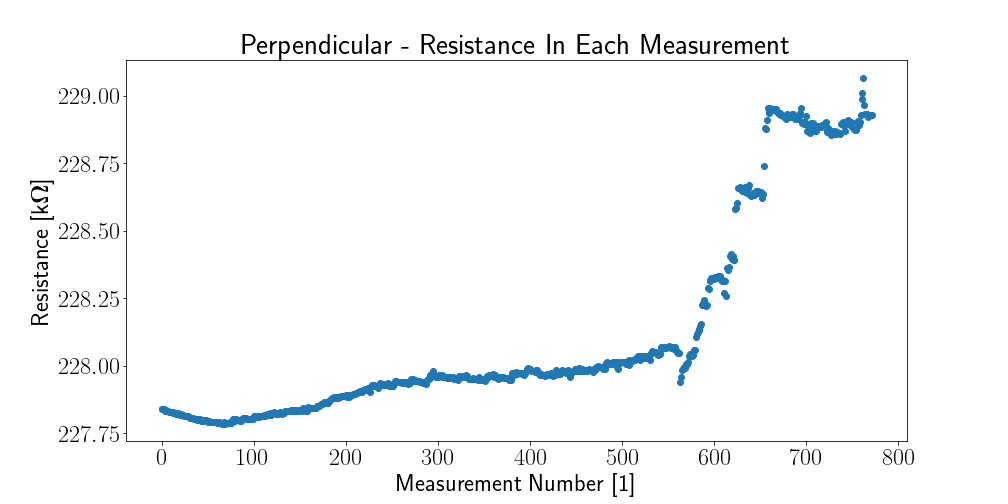
\includegraphics[scale=0.23]{Measurements/Graphs/AMR-PerpVsTime}

\caption{Measured resistance plotted against measurement number \label{fig:AMR-Resistance-Time}}
\end{figure}

the resistance measurements are not accurate to an order of $1\,k\Omega$
, and so, the difference is of the magnitude of the system's resolution,
i.e. $1\,k\Omega$. The change in the resistances of the transverse
and the parallel fields are inconsistent with the theory. The transverse
field saturates at a higher resistance than it started at and is not
monotonic. In addition, the parallel field saturates at a lower, rather
than higher resistance and monotonically decreases as opposed to increasing.
Both graphs contradict Figure \ref{fig: AMR_MagnetoResistance}. There
are two possible explanations for these results. The first, that a
mix-up between the two measurements was made, however, that is highly
unlikely as the measurements were done in separate excel files, meaning,
the mistake had to happen twice. The second explanation is that the
connections were faulty, or that the wrong connections were made.
\\
By looking at the symmetric parts and estimating at which field strength
the average resistance no longer changes, the field required to saturate
the magnetization along that axis is found. Our estimates are $H_{sat}^{P}\approx3000\,[Gauss]$,
$H_{sat}^{T}\approx2500\,[Gauss]$ and $H_{sat}^{\parallel}\approx2000\,[Gauss]$,
these suggest that the hard axis of the fcc crystal is mostly along
$\hat{z}$, and the easy axis is mostly along $\hat{x}$. This finding
is opposed to the result in the AHE which suggests that the easy axis
is mostly along $\hat{z}$, this may also corroborate the hypothesis
that the measurements of the parallel and transverse parts were mixed
up or that the connections were faulty.

\section{AHE}

The extracted values from the anomalous Hall effect are of the same
scale as values from the literature and as can be seen in Figure \ref{fig: AHE linear fits}
a clear hysteresis loop can be seen and both the normal and anomalous
Hall effects can be observed. The saturation magnetization may  have
been smaller or bigger than its final value as the way it was estimated
 offers freedom and allows to perform linear fits with data from
different regions, yielding different intersection points and thus
different saturation magnetizations. In this part of the experiment,
the external magnetic field was directed perpendicular to the plane
of the nickel sample, along $\hat{z}$ , and the coercivity and width
of the hysteresis loop align with values corresponding with those
belonging to the easy axis of nickel, which suggests that $\hat{z}$
is the easy axis of the material. As was mentioned in the AMR section,
there is a difference between the results from AMR and the results
from this experimental part, which can be attributed to faulty connections
of the experimental system as the results from AMR prove significantly
different from the expected theoretical behavior. Regardless of the
inability to extract convincing information about the sample from
the AMR section, both PHE and AHE support the claim that the easy
axis lies in the $z$ direction. 

\bibliographystyle{plain}
\bibliography{Report}

\end{document}
